\chapter{Opportunistic Relaying}
\label{chap:opp_relay}

\section{Background}
Wireless network providers are under tremendous pressure to deliver unprecedented amounts of data to a variety of mobile devices. A powerful concept that has only gained limited traction in practice has been the concept of opportunistic networks whereby nodes opportunistically communicate with each other when in range to augment or overcome existing wireless systems. Although opportunistic networking has received more attention as of late with the rise of various point-to-point technologies (WiFiDirect, LTEDirect) directly embedded in user devices, traction in terms of significant adoption remains elusive as the mere existence of point-to-point wireless technology is insufficient.  Rather, infrastructure support (albeit at a software or protocol level) is still required that is impeded by the lack of shared, longitudinal data taking a serious look at the potential for opportunistic relaying amongst actual mobile device users to justify said investment in infrastructure. The actual gathering of said data though is in and of itself quite difficult, requiring one to overcome numerous issues with respect to privacy, cost, scale, and quite simply the amenability of the device to acquire said data. Thus, in the absence of real data and the difficulty in acquiring such data, opportunistic networking research has largely espoused synthetic or theoretical explorations of user mobility.  In this Chapter, we demystify the opportunities that exist for opportunistic relaying by bridging the gap with our large scale dataset. 

\section{Related Work}\label{sec:related_work}
The notion of what constitutes an \emph{opportunistic communication} encompasses a wide variety of research and standardization efforts within the networking community.  From the more traditional perspective, opportunistic relaying represents wireless nodes taking advantage of emergent opportunities to relay data towards its eventual destination originally espoused by~\cite{laneman2004cooperative} and expanded up by numerous others \cite{bletsas2006simple,lu2009design,bahl2009opportunistic}.  More recently, considerable efforts have emerged where IEEE 802.11-based networks (WiFi) are viewed through an opportunistic viewpoint, espousing the delay of packets to favor the potentially faster WiFi over the congested cellular link.  More aggressive variants include `Opp-Off' as proposed in~\cite{han2011mobile2} which intentionally delays the delivery of information over cellular networks and offload it through the `free' opportunistic communications. Similarly, in~\cite{dimatteo2011cellular}, another delay-tolerant network (DTN)-like architecture called `MADNet' is proposed by integrating WiFi networks and mobile-to-mobile Pocket Switched Networks (PSN) with cellular networks.   With the ability to leverage the availability of inexpensive 802.11, both Opp-Off and MADNet are able to conduct real-world experiments on live systems, albeit on a limited scale and time period.   

A key foundation for the evaluation of opportunistic networks arises from the characterization of inter-contact times 
~\cite{chaintreau2007impact,cai2008toward,lee2009slaw,karagiannis2010power,passarella2011characterising}. The work in \cite{chaintreau2007impact} was one of the first works to highlight the importance of inter-contact for studying opportunistic networks and analyze the features of aggregate inter-contact times. In the work of~\cite{cai2008toward,lee2009slaw}, the mobility models proposed for opportunistic networks aim at reproducing the aggregate power-law distributions.  The mobility models in turn provide powerful abstractions for the evaluation of various theoretical properties of opportunstic networks that is critical for understanding general limits of the overarching relay protocols.  In contrast from these studies on statistical patterns of human mobility, we focus on the analysis to take in not only the proximity into consideration but also other elements such as traffic needs and battery influences which have to the best of our knowledge, not explored in a unified manner in the literature. 

\section{Evaluating Practical Relaying}\label{sec:potential}

The dataset outlined in Chapter~\ref{chap:dataset} provides a fascinating opportunity to evaluate the actual prevalence with respect to opportunistic relaying in the `wild' evaluating not only the prevalence itself but when intra-study proximity is involved, significant explorations with respect to the mutual benefits of relaying or collaborative efforts.  For the purposes of evaluation, we are concerned with two types of opportunistic networking, namely relaying and collaboration.  In the first case of relaying, a mobile node ($MN_i$) might relay the traffic from mobile node ($MN_j$) when $MN_j$ has a weak / non-existent wireless signal or $MN_i$ has a good signal to a preferred wireless medium (ex. WiFi) while $MN_j$ does not.  In the second case of collaboration, $MN_i$ and $MN_j$ work together to overcome a lossy channel either by the use of striping across both nodes (ex. auxiliary relaying of TCP ACKs \cite{SteenkisteRelayACK}) or striping across different wireless mediums (WiFi + cellular).  Opportunistic communications would be provided through mobile-to-mobile communications (Bluetooth, WiFiDirect, LTEDirect). Both approaches to opportunistic relaying would require modifications to the wireless infrastructure as well as security concerns to establish any mobile-to-mobile communication which are beyond the scope of this paper.  Rather, we focus on the more fundamental question of \emph{does enough opportunity exist} and if so, \emph{is it of reasonable quality to make it worthwhile}?  

\begin{landscape}
\begin{table*}[t] 
\caption{FRAMEWORK FOR EVALUATING AVAILABILITY, PREVALENCE, STABILITY, RECIPROCITY} 
\centering
\begin{tabular}{l|p{3.5cm}|p{1.5cm}|p{11cm}}
\hline
\multicolumn{2}{c|}{Criteria} & \multicolumn{1}{c|}{Term} &\multicolumn{1}{c}{Description}  \\ 				
\hline
\hline  
\multirow{5}{*}{Availability}   & Sufficient Signal & $SS$ 	& `good signal' to indicate proximity  \\ 
\cline{2-4}		 			  & Symmetry & $Sym$		& Time when proximity is symmetric, has $SS$ vs. time powered on \\
\cline{2-4}		  		           & Diversity & $Div_n$	         & Time with at least $n$ nodes with $SS$ detected vs. time nodes detected \\ 
\cline{2-4}					  & Residual Battery & $RB$	& Time with proximity of other nodes with $SS$ and enough battery to do relaying vs. time with proximity \\

\hline  
\multirow{2}{*}{Prevalence}   & Time in Proximity & $TIP$ 	& Time with proximity vs. time powered on  \\ 
\cline{2-4}					  & Intercontact Time & $IT$	& Time between two successive contact/proximity periods \\
\cline{2-4}					  & Effective Utility & $EU$	& Time with proximity of other nodes with $SS$, $Sym$, traffic to send vs. time with traffic to send \\

\hline \multirow{4}{*}{Stability} 		& Duration & $D$			& Number of consecutive contact durations vs. instances of contact at $MN_i$ \\
\cline{2-4}			     			&  Node Strength & $NS$	&  Number of total appearances by $n$ most common peers \\
\cline{2-4}			     			&  Total Appearances & $TA$	& Number of appearances of a device vs. total device appearances at $MN_i$ \\
\cline{2-4}			     			&  Continuous Appearances & $CA$	& Number of consecutive appearances of a device vs. appearances of multiple days at $MN_i$ \\
\hline \multirow{4}{*}{Reciprocity}  & Need Service & $Serv$ & Time when no auxiliary WiFi is present and traffic demand exists vs. time powered on\\
\cline{2-4}	  		       		 & Offer Assistance & $Assist$ & Time ween detected with $SS$ vs. time powered on 	\\
\cline{2-4}					 & Ratio Need vs. Assist & $R_{NA}$ & Time of $Serv$ vs. Time of $Assist$ \\ 
\hline
\end{tabular}
\label{table:metrics} 
\end{table*}
\end{landscape}

To that end, we seek to answer the following questions in this section of the paper summarized in terms of metrics in Table \ref{table:metrics}:

\begin{itemize}
	\item \emph{Availability}: How is proximity defined and what criterion should exist to enable opportunistic communication with respect to inter-node communications?  What can be considered a `good' opportunistic link in terms of the underlying physical link quality and at what granularity is such data recorded? How does the residual battery influence the potential for relaying? 
	\item \emph{Prevalence}: What is the frequency that a mobile device detect other devices in proximity?  To what extent is the detection symmetric for intra-study participants?  How does the inter-contact times of nodes compare to prior work?  Do opportunities exist when needed (traffic demand) making them useful versus simply available?  
	\item \emph{Stability}: To what extent are discovered opportunities stable enough that an overarching security mechanism could complete or relevant data exchanges could take place?  Are there consistent patterns with regards to nodes appearing more common than others allowing expedited trust?   
	\item \emph{Reciprocity}: Even if opportunities are shown to be prevalent and stable, to what extent are the relationships likely to be reciprocal, namely both $MN_i$ and $MN_j$ will benefit on average equally in terms of both receiving assistance and giving assistance?  When energy is factored in as a consideration for nodes not being willing participants, does any sort of prevalence or reciprocality disappear?  Finally, reciprocality if it exists, does it exist exclusively in only longer-time scales or does it exist on reasonably short-time scales as well?    
\end{itemize}

For the wireless network, we first being by defining several key attributes of the data.  Each mobile node ($MN_i$) is considered to have a discrete set of samples at periodic intervals capturing the proximity of nearby nodes (Bluetooth), the signal strength from each detected Bluetooth node as received at $MN_i$, (ex. $MN_j \rightarrow MN_i$), each detected AP and also the signal strength for each AP as detected by $MN_i$ by virtue of the beacon signal strength.  Each time slot is assumed to be five minutes long (for the purposes of assessing if the phone was on or off) though durations of contact are calculated using per-minute measurements.  The term \emph{Good RSSI} refers to thresholds for RSSI values that indicate the potential for excellent performance although in practice such performance may vary.  Performance with respect to each node is normalized unless explicitly noted to the actual time that the phone was on (powered on, agent running) for that particular day or period. 

\subsection{Availability}
The first question to pose is how to define proximity. We begin with the most basic question with regards to the signal strength of discoverable Bluetooth devices and detected APs and further refine our queries to explore various aspects of availability through the Availability criterion of the APSR framework. 

\subsubsection{Proximity}
As demonstrated in Chapter~\ref{bt_proximity}, we use Bluetooth as the proximity mechanism for multiple reasons.  First, the effective range of Bluetooth typically is on the order of 10m or less.  In contrast with other point-to-point technologies such as WiFiDirect and LTEDirect which have the potential for significantly longer ranges, Bluetooth in effect represents a minimum or floor to the potential for opportunistic communications as the various *Direct technologies would easily be able to cover the 10m effective range of Bluetooth.  Second, although Bluetooth is reasonably common amongst smart phones, the locking of a device as being discoverable is fairly uncommon, largely for reasons of security.  Despite the somewhat uncommon nature of discoverable Bluetooth (most devices require specific action to make themselves discoverable), a robust finding even with the limits of Bluetooth discoverability represents again a floor or minimum potential available.  Critically, the act of gathering Bluetooth discoverable devices is reasonably power efficient allowing one to gather available devices at a reasonable pace (with associated signal strength for Bluetooth) without pairing and while still having a reasonable device battery life for the study. 

Notably, the mere existence of the device being discoverable does not necessarily imply that the point-to-point link will be suitable for opportunistic communications.  Figure~\ref{fig:rssi} shows the ECDF of the Bluetooth RSSI values in different months and more than 60\% of the values are larger than -80dBm.  In particular, the data of July 2012 consider all the records including the Bluetooth devices outside the project and APs not under university control. Based on the work in ~\cite{polastre2005telos}, the RSSI value \emph{-80dBm} is used as a threshold to indicate good Bluetooth RSSI for direct mobile-to-mobile communication.  

\begin{figure}[tbp]
\centering 
{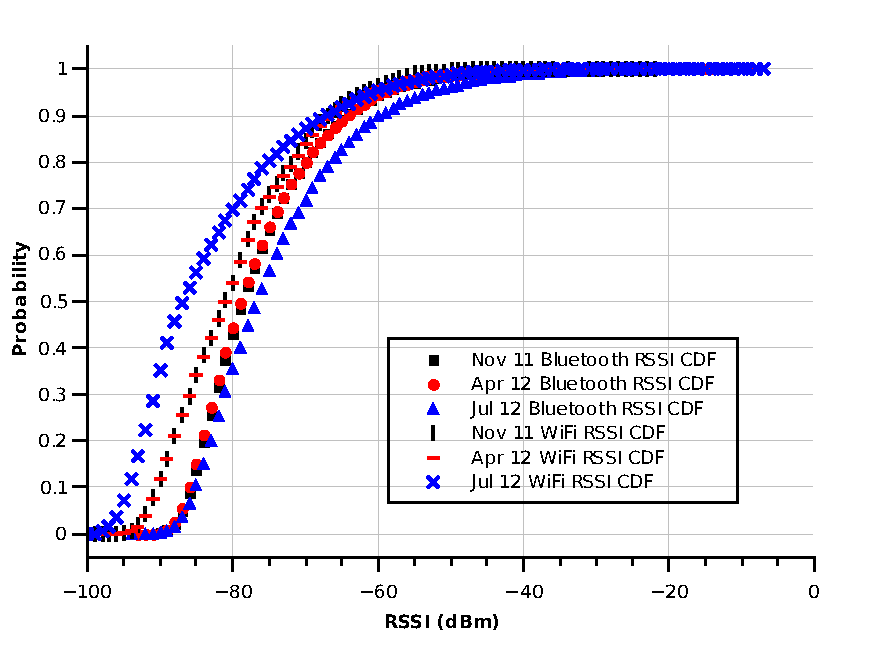
\includegraphics[width=3.5in]{graphs/rssi.pdf}}
\caption{Bluetooth and WiFi RSSI Values ECDF} 
\label{fig:rssi}
\end{figure} 

While Bluetooth is used in the first part of the section to assess proximity, to what extent could we infer proximity if we expanded our search to consider common detected WiFi APs.  For instance, in ~\cite{mcnett2005access}, WiFi signal strength is used to indicate proximity when two devices are associated to the same AP.  We further restrict the characterization to infer proximity if two mobile nodes detect two or more same access points.  Barring the two APs being situated nearly on top of one another (note that university APs are filtered down to disambiguate virtual APs), one can reasonably infer that two nodes sharing the same two or more APs could be in WiFiDirect and / or LTEDirect range. Figure~\ref{fig:bt_wifi_distribution} shows the ECDF of Bluetooth proximity percentage and WiFi proximity percentage. The percentage of time represents the percentage of time where an opportunity might exist for collaboration either within Bluetooth proximity or WiFi proximity. Interestingly, the WiFi result conveys less proximity than the noted Bluetooth proximity.  The discrepancy can be traced to one primary culprit, namely the poor signal reception of smartphone WiFi adapters as originally noted by \cite{liu:CellNet12}.  Notably when compared to reference laptops or tablets, the work in \cite{liu:CellNet12} notes a roughly 10 dBm signal penalty for the smartphone.  The net result is in addition to the detection of WiFi APs being hampered, reasonable placement of APs and auto-tuning of AP strength would result in significantly reduced probabilities of multiple mobile devices being able to detect one or more APs. In Figure~\ref{fig:wifi_fp_fn0}, we compare the results of WiFi proximity and Bluetooth proximity in April of 2012 and November of 2011. The false positive means the device detects other(s) in WiFi proximity which are not detected by Bluetooth proximity. On the other hand, the false negative means that the device does not detect some device in WiFi proximity but does detect the device in Bluetooth proximity. Notably, the false positive in the context of WiFi may not be a false positive but the false negative most certainly represents an incorrect result due to the aforementioned signal holes noted in \cite{liu:CellNet12}.  

\begin{figure}[tbp]
\centering 
{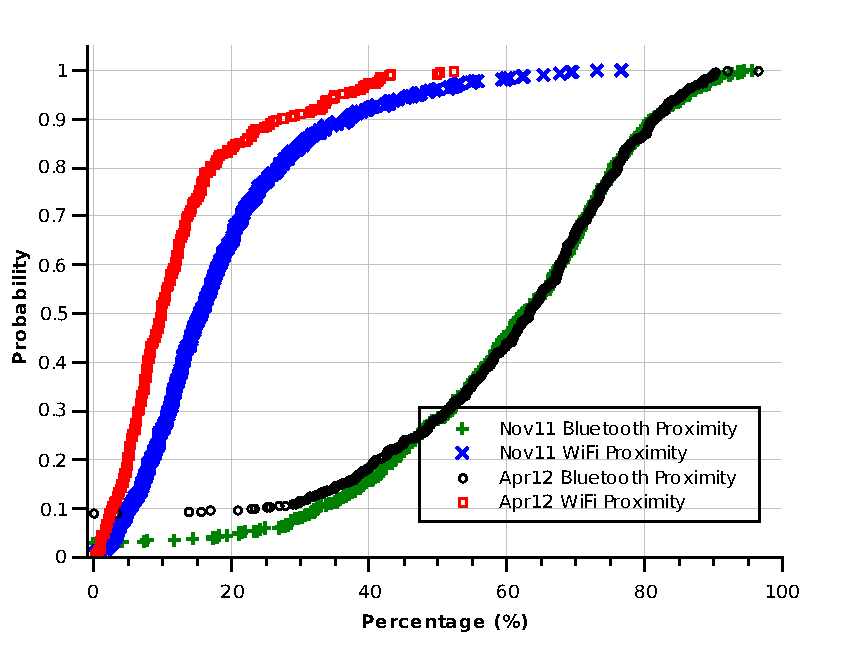
\includegraphics[width=3.5in]{graphs/bt_wifi_distribution_201204.pdf}}
\caption{Bluetooth Proximity and WiFi Proximity ECDF in April 2012} 
\label{fig:bt_wifi_distribution}
\end{figure} 

\begin{figure}[tbp]
\centering 
{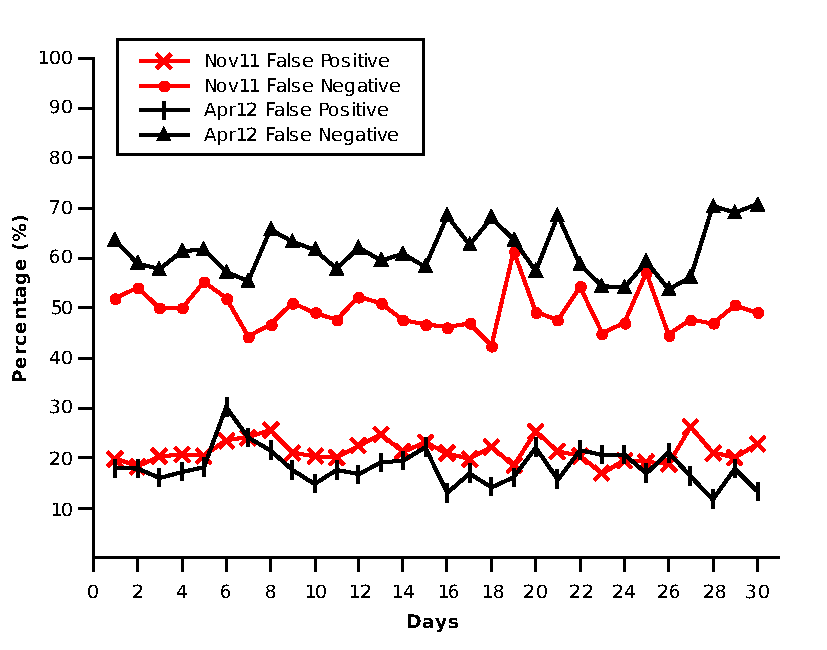
\includegraphics[width=3.5in]{graphs/wifi_falsenegative.pdf}}
\caption{Comparison of Bluetooth Proximity and WiFi Proximity} 
\label{fig:wifi_fp_fn0}
\end{figure} 

\subsubsection{Symmetry}

Symmetry is defined as both nodes seeing each other in proximity. For WiFi proximity, such symmetry is 100\% based on its definition. However, for any two study participants in Bluetooth proximity, there exists the opportunity to determine if detection symmetric exists, namely do both nodes detect each other and even if both nodes detect each other, do both nodes have a `Good RSSI' to one another ($MN_i \rightarrow MN_j$ and vice versa)? In Figure~\ref{fig:daily_symmetric}, the symmetry of Bluetooth proximity within study with `Good RSSI' is illustrated by using the data in November 2011 and April 2012. Notably, roughly one third of the opportunities disappear due to the consideration of symmetry. Many reasons may cause the asymmetry such as environment inference and it is quite expectable in practice. 

\begin{figure}[tbp]
\centering 
{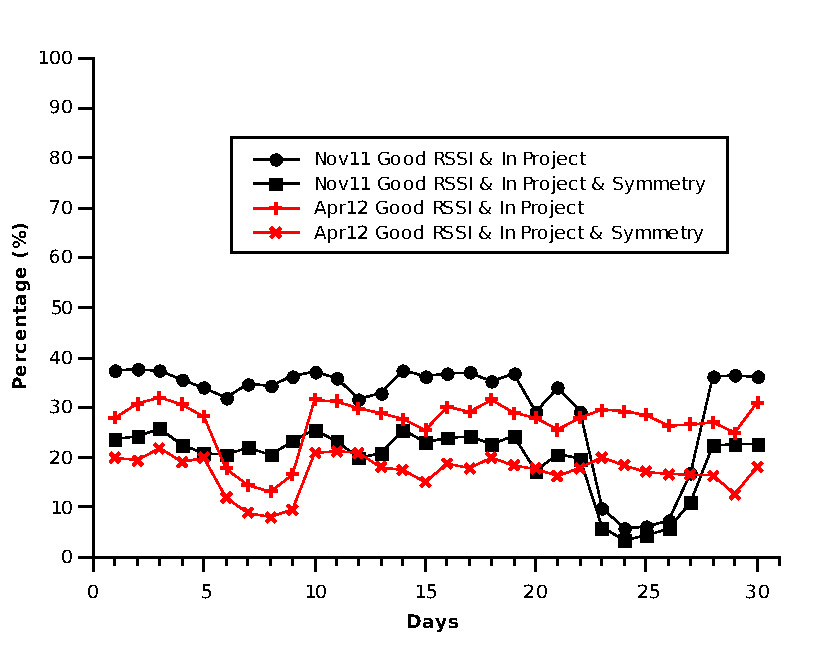
\includegraphics[width=3.5in]{graphs/daily_symmetric.pdf}}
\caption{Symmetry of Bluetooth Proximity} 
\label{fig:daily_symmetric}
\end{figure} 


\subsubsection{Diversity}
While symmetry represents just one part of the puzzle, an related factor for the opportunity to be useful is with regards to the diversity of opportunities available.  Relaying selection plays little role when there exists only a single device to choose from for relaying.   Figure~\ref{fig:relay_num} shows the breakdown of detected devices in proximity through both Bluetooth and WiFi in April 2012 representing only cases where proximity occurred. In the figure, nearly 60\% of time has only one peer is detected among all the possible opportunistic time slots. Meanwhile, there is nearly 20\% of the time when two opportunities are detected and finally 20\% when three or more opportunities are detected. In Figure~\ref{fig:relay_num_diurnal}, more details about the number of detected devices in April 2012 is illustrated with a diurnal distribution across the same month breaking down only cases where proximity was detected, i.e. 50\% of daytime detections involved only a single device in the study. During the daytime, the chance to detect two or more devices in proximity is higher than other durations. Again, day time offers an increased potential for diversity in large part due to the increased mobility around the campus.  

\begin{figure}[tbp]
\centering 
{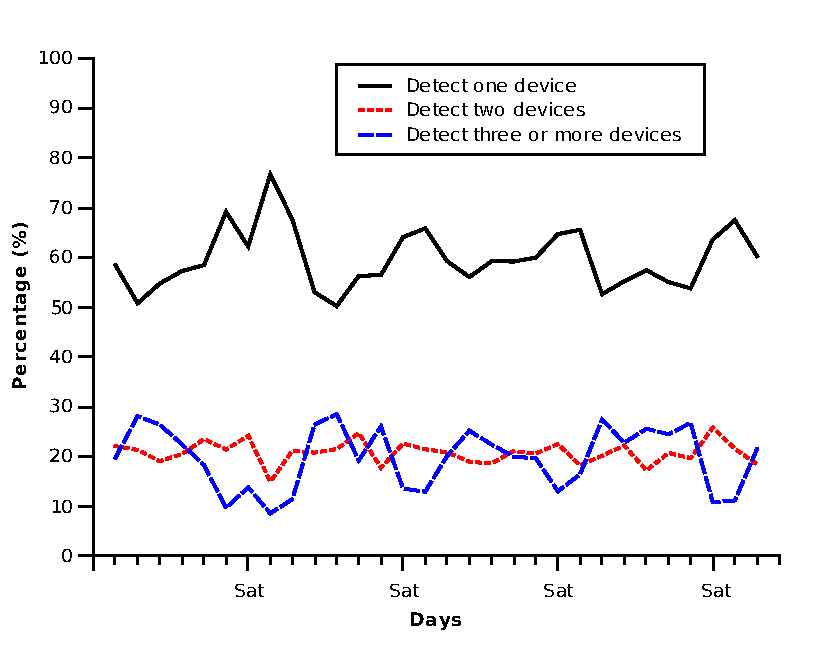
\includegraphics[width=3.5in]{graphs/relay_num.pdf}}
\caption{Distribution of Proximity Diversity (In-Study) in April 2012} 
\label{fig:relay_num}
\end{figure} 

\begin{figure}[tbp]
\centering 
{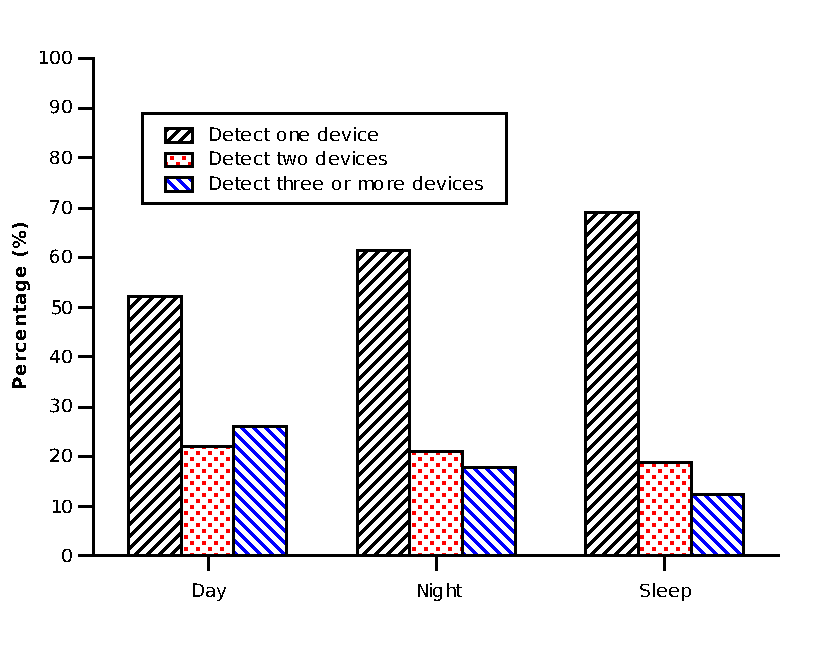
\includegraphics[width=3.5in]{graphs/relay_num_diurnal.pdf}}
\caption{Diurnal Distribution of Proximity Diversity in April 2012} 
\label{fig:relay_num_diurnal}
\end{figure} 

As mentioned before, it is fairly uncommon making the device Bluetooth discoverable. In order to reveal the diversity of potential relaying nodes, we investigate the types of available Bluetooth devices in proximity based on the Bluetooth data across the study. There are around 49\% of distinguished Bluetooth discoverable devices are smartphones. Interestingly, 10\% of the devices are Apple products: 80\% of them are iPhone/iPod/iPad, and rest of them are Macbook laptops. 

\subsubsection{Residual Battery}
The availability of opportunistic communication depends on not only the existence of devices in proximity, but also the battery status of detected devices, i.e. making sure the relaying devices have enough residual battery for the following communication. As discussed in~\cite{zou2012exploiting, madan2008energy}, residual battery is an important consideration factor for relaying selection. Even the device is detected in proximity, it cannot be utilized for relaying if the battery is too low to do transmission. At the same time, it is the basic premise for device having enough energy for communication when it detects other devices in proximity. 
Due to the battery data collection limitation, we focused on the devices within the project and analyzed the percentage of Bluetooth proximity when the battery level is low (i.e. level value smaller than 30) and the result is shown in Figure~\ref{fig:battery}. In April 2012, daily power on time is around 18 hours on average and the low battery time when the devices are in proximity scenarios is nearly 1 hour. Meanwhile, the average time of detecting proximity and being detected as proximity is around 7 and 5 hours. Therefore, the percentage of low battery time is relatively small and 

\begin{figure}[tbp]
\centering 
{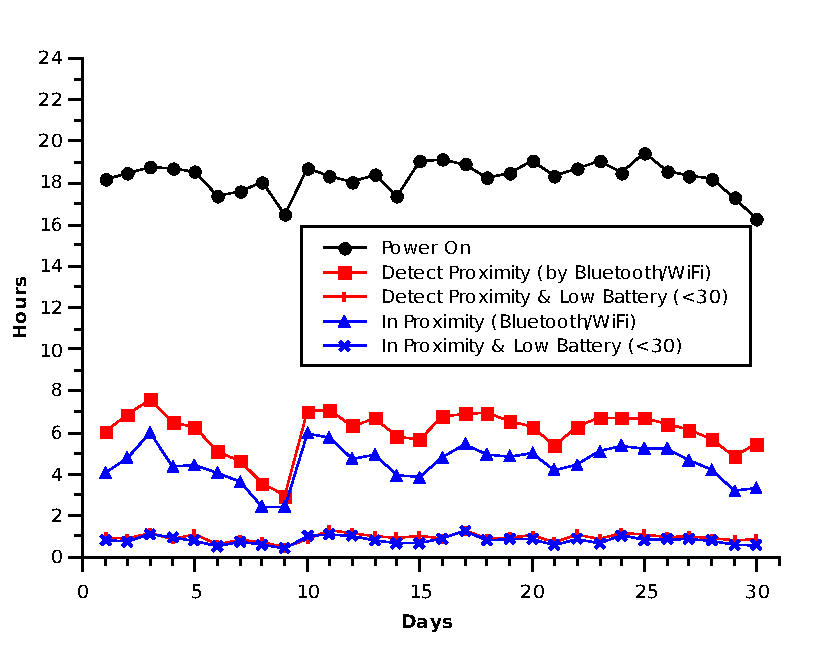
\includegraphics[width=3.5in]{graphs/battery.pdf}}
\caption{Average Daily Low Residual Battery Time in April 2012} 
\label{fig:battery}
\end{figure} 

\subsubsection{Evaluating Availability} 

To summarize, we conclude availability of opportunistic communication with a brief discussion of metrics used to evaluate availability.
\begin{itemize}
	\item Sufficient Signal: While the use of all available proximity potentially may be of interest, only useable mobile-to-mobile links are of interest.  An explicit filter likely unique to each particular handset or device should be employed.  
	\item Symmetry: Filtering the data further, agents monitoring the signal strength on both sides of the dyadic pair can assess if symmetry exists both with respect to detection ($MN_i$ detects $MN_j$, vice versa) and sufficient signal strength.  
	\item Diversity: When there are more than one relaying nodes nearby, it is easier for the device to choose one of the most appropriate nodes with the consideration of benefits on both sides. 
	\item Residual Battery: As an important criterion for relaying selection in various relaying protocol, battery of mobile devices is essential for availability. When the residual battery of mobile devices is low, it is difficult for the devices to do opportunistic communication.  
\end{itemize} 

\subsection{Prevalence}\label{sec:prevalence}
Availability analysis exhibits the possibility to detect other devices in proximity. A more important question is to what extent such opportunistic communication opportunities exist in practice.  We begin with the most basic question with regards to the prevalence of discoverable Bluetooth devices and further refine our queries to explore various aspects of prevalence through the Prevalence criterion of the APSR framework.  We posit several questions that include: (1) the extent to which discoverable Bluetooth devices exist, (2) the extent to which WiFi proximity exist, (3) and the extent to which diurnal (daily) patterns play a role in discoverable devices.  We further continue the explorations examining the prevalence of proximity to determine if the prevalence of such opportunities are still useful, namely (1) are such opportunities only available when there is no traffic and (2) how frequent do opportunities exist to augment access to `better' wireless channels (ex. WiFi).   

\subsubsection{Time in Proximity}
Based on the 15 months data, Figure~\ref{fig:bluetooth} illustrates the average weekly Bluetooth proximity percentage with different restrictions across the study period.  Various periods of interest representing various break periods are labeled in the graph. Further restrictions are placed on the data to filter for `good RSSI' and candidates for opportunistic communications to exist only within the project (study).   Notably, when completely unrestricted opportunities exist on the average of nearly 60\% of the time when on campus, falling only slightly when good signal strength is added as a restriction.  Even intra-study opportunities are quite prolific despite the fact that the 200 study participants represent less than one tenth of the freshmen class and less than 2.5\% of the overall university student population.With the threshold of -80dBm for the `Good RSSI', there still exists more than 50\% of the time slots, a fairly insubstantial drop from the raw detected Bluetooth devices. The slight drop from the fall of 2011 to the fall of 2012 can largely be attributed to students joining their respective majors and having less shared coursework versus their freshmen year.  Moreover, we compare Bluetooth proximity with and without consideration of symmetry. Similarly as the results in Figure~\ref{fig:daily_symmetric}, the one third drop rate due to asymmetry is quite stable across the study.  Although the lack of symmetry does temper the earlier findings of prevalence, we note that Bluetooth is most appropriately viewed as a floor for potential interactions.  The potential for asymmetry though between nodes does represent a consideration that merits further attention.  

\begin{figure}[tbp]
\centering 
{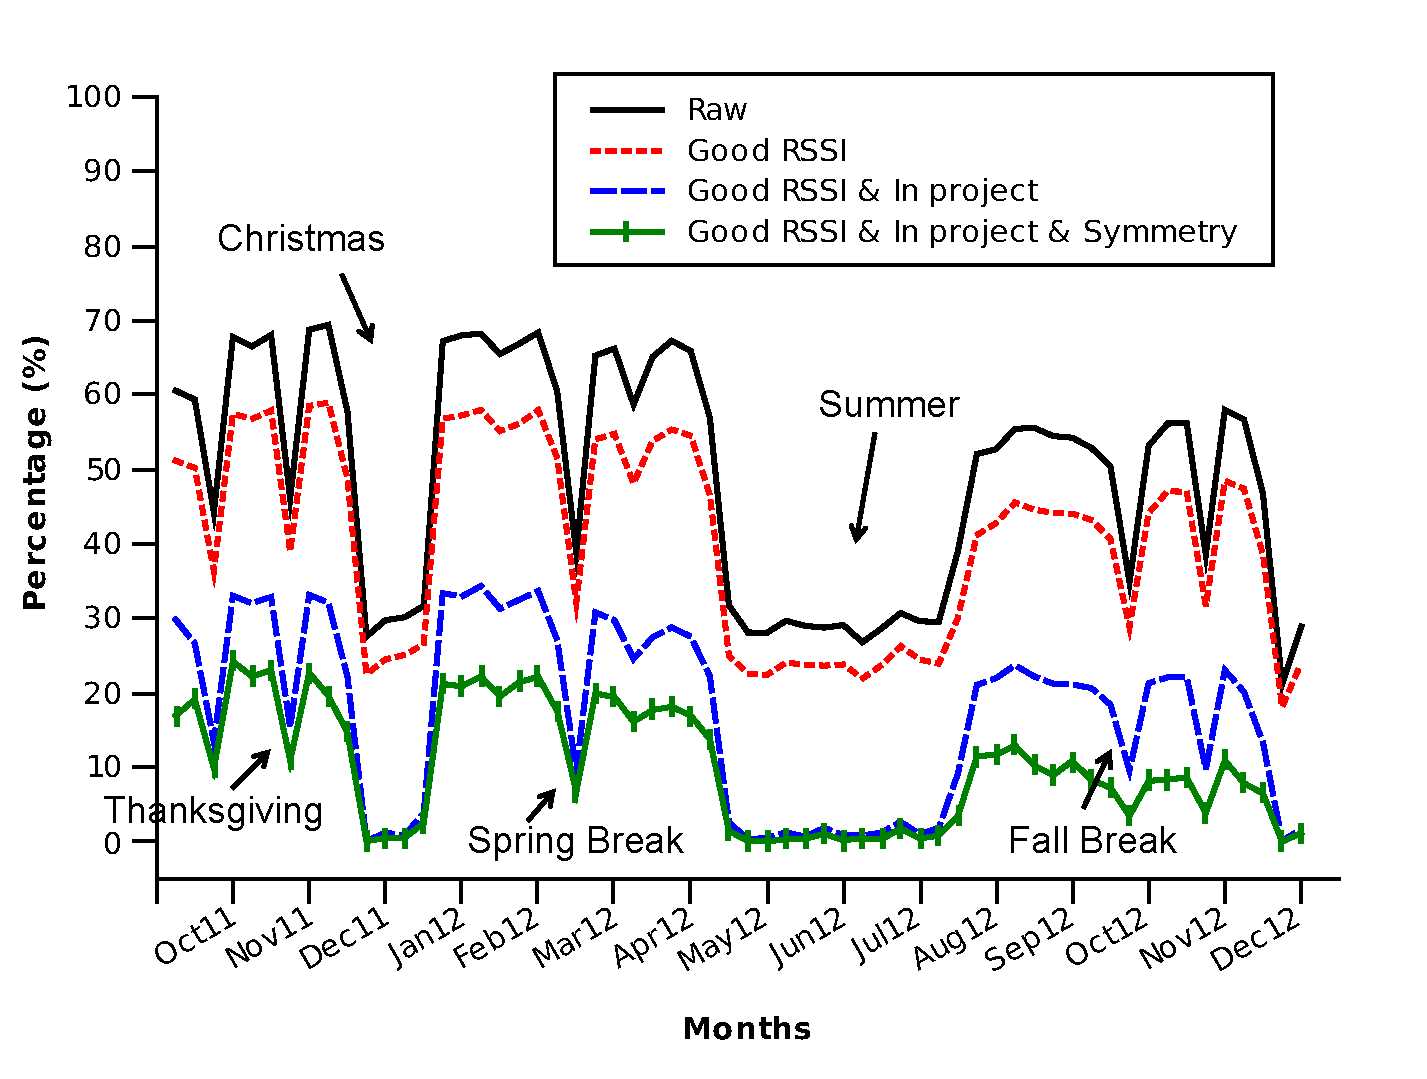
\includegraphics[width=3.5in]{graphs/weekly_bluetooth_with_symmetry_tag.pdf}}
\caption{Bluetooth Proximity with Different Restrictions} 
\label{fig:bluetooth}
\end{figure} 

Given that the students were selected from a core group of six dormitories, a natural skepticism should emerge from the data with regards to the diurnal effects of proximity, namely proximity does little good if it only occurs at night when the phone is not otherwise being used (ex. sleeping in the dorm room).  Hence, we analyze the diurnal distribution of Bluetooth proximity by dividing one day into three parts: day time (8am to 4pm), night time (4pm to 12am) and sleep (12am to 8am). In this way, we are able to investigate the impacts of time durations on such proximity. Figure~\ref{fig:diurnal} shows the diurnal distribution with the twin restrictions of good RSSI and intra-study detected proximity only. The daytime proximity percentage from 8am to 4pm is larger than the value during nighttime and almost equal to the value of sleep time.  The separation from in the fall of 2012 largely follows the classroom / major separation as noted in the raw and restricted graphs. 

\begin{figure}[tbp]
\centering 
{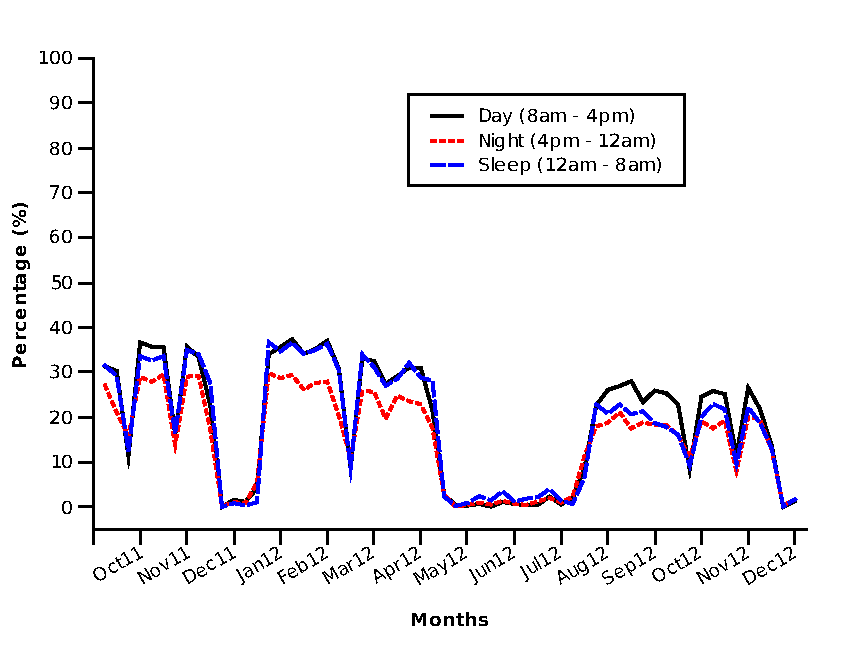
\includegraphics[width=3.5in]{graphs/weekly_bluetooth_diurnal.pdf}}
 \caption{Diurnal Distribution of Bluetooth Proximity} 
\label{fig:diurnal}
\end{figure} 

Beyond coarse diurnal metrics, significant day of week effects can also exist. Course patterns can vary dramatically between the Monday / Wednesday / Friday courses and Tuesday / Thursday courses.  Similarly, weekends are much more likely to be quite diverse from normal weekday patterns.  Figure~\ref{fig:diurnal_april} shows the daily Bluetooth proximity and diurnal distribution in April 2012 for a more detailed comparisons among the weekdays with each respective Saturday noted on the x axis. The peak values always appear at the beginning of the week and decrease slowly during the week. During the Easter holiday (April 6th - April 9th), the opportunities for proximity shrink dramatically as the students travel home for Easter break. Meanwhile, more Bluetooth proximity appeared in the later hours (broadly defined as sleep time) than daytime hours during weekend which indicates the participants spent more time in closer proximity to others during those time periods largely as a byproduct of social relationships. 

\begin{figure}[tbp]
\centering 
{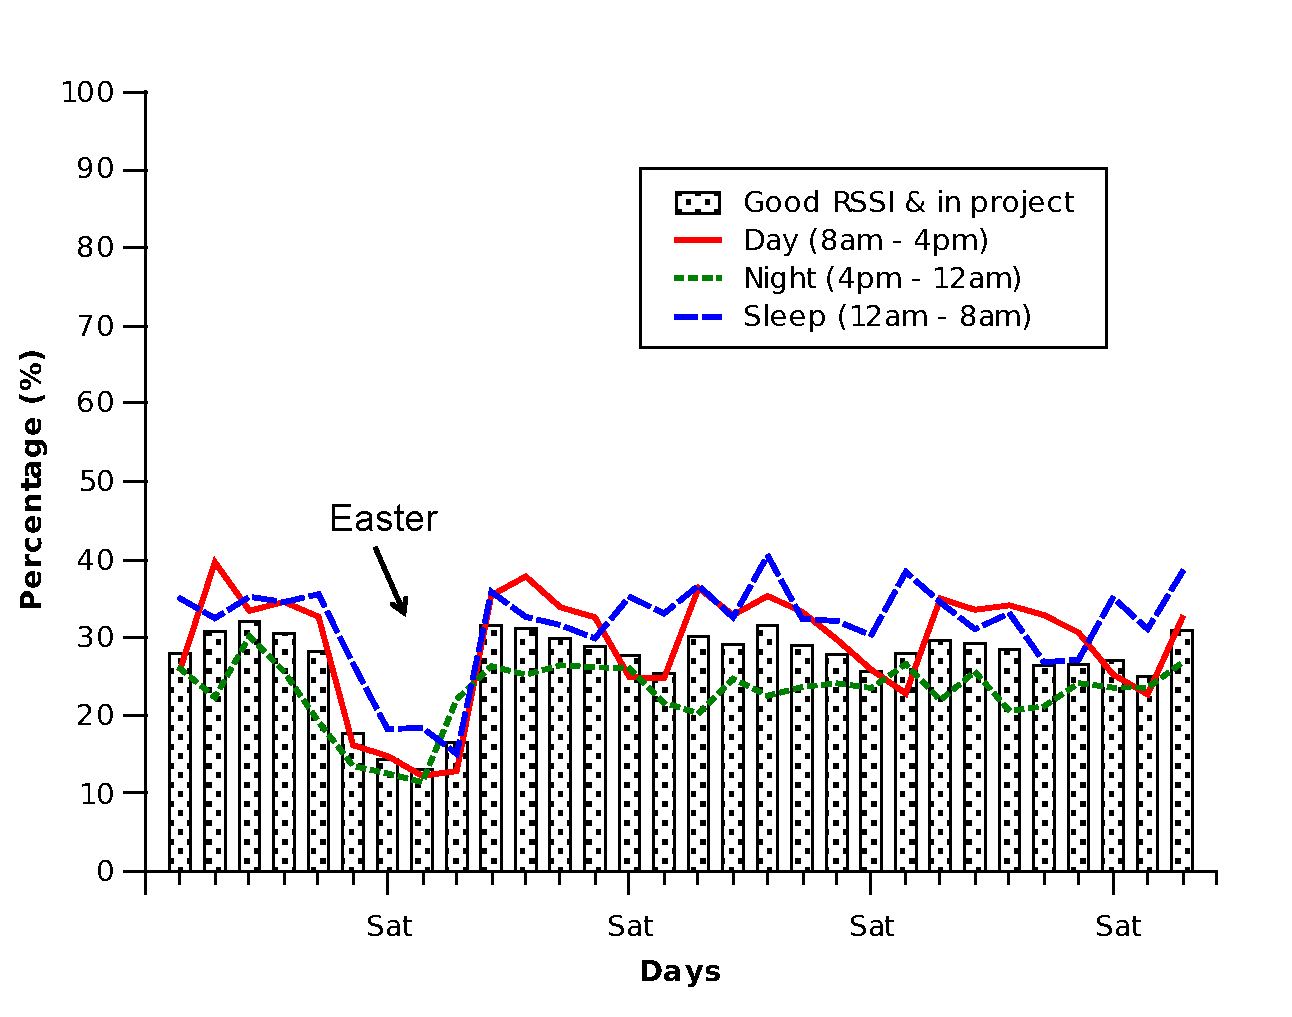
\includegraphics[width=3.5in]{graphs/bluetooth_201204_tag.pdf}}
\caption{Diurnal Distribution of Bluetooth Proximity in April 2012} 
\label{fig:diurnal_april}
\end{figure} 

For WiFi proximity, we analyze the number of time slots when the device shares at least two of the same access points with another device (in-study devices only) and we calculate the percentage of such time slots. Figure~\ref{fig:wifi} demonstrates the WiFi proximity and its diurnal distribution across the study period. During the holidays and summer, the percentage is almost zero as only university APs are considered for WiFi performance. Compared to other periods, WiFi proximity during daytime from 8am to 4pm represents a slight uptick though not statistically significant variation over other periods. 

\begin{figure}[tbp]
\centering 
{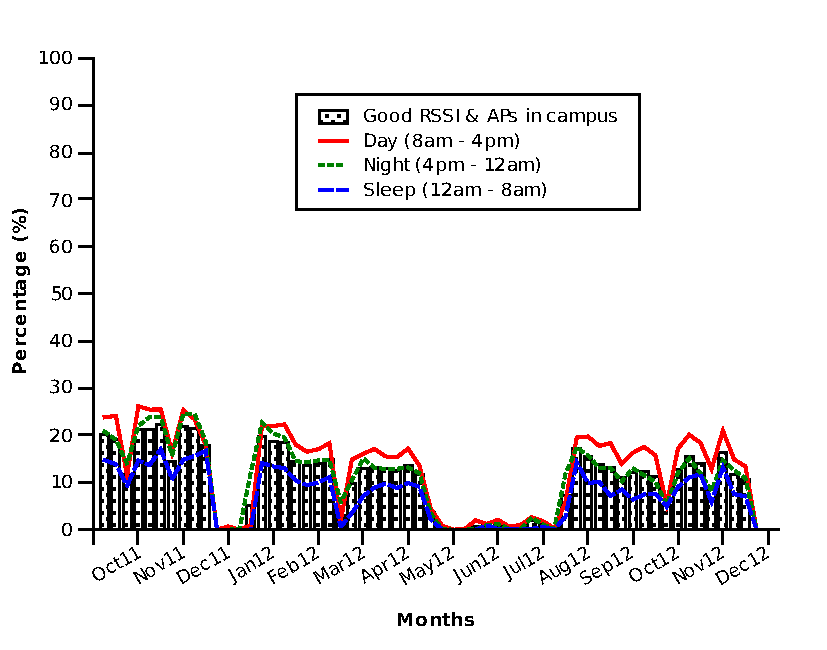
\includegraphics[width=3.5in]{graphs/weekly_wifi.pdf}}
\caption{WiFi Proximity} 
\label{fig:wifi}
\end{figure} 

Taking a bit more of an optimistic stance, we combine both WiFi proximity detection and Bluetooth proximity detection to create a combined proximity.  Note that earlier proximity measurements used either exclusively Bluetooth or WiFi.  Broadly defined, in one specific time slot, if the device can either detect other devices within the project with good Bluetooth RSSI or share at least two same APs in the campus with good WiFi RSSI, this time slot is counted as one of the slots when the device is in proximity with another device (intra-study only). Figure~\ref{fig:bt_wifi} illustrates such proximity across months. Compared to Bluetooth proximity only or WiFi proximity only, the percentage is increased to more than 40\% trailing to roughly 30\% by the end of the study, a nearly 10\% increase over Bluetooth only considerations. The diurnal distribution keeps the same trend and the proximity percentage during the daytime being is the highest among the respective time periods.

\begin{figure}[tbp]
\centering 
{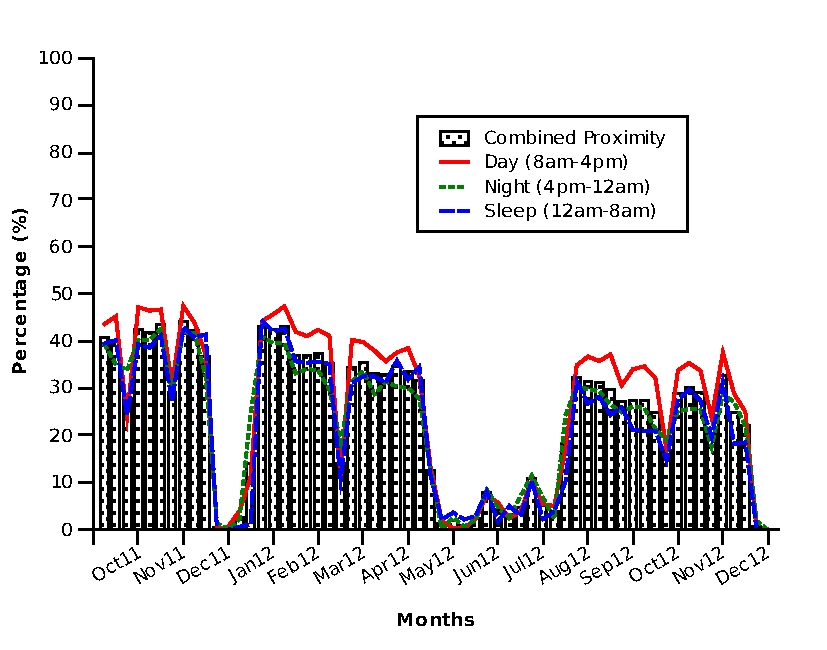
\includegraphics[width=3.5in]{graphs/weekly_bt_wifi.pdf}}
\caption{Combined Proximity (Fused Bluetooth / WiFi Detection)} 
\label{fig:bt_wifi}
\end{figure} 

\subsubsection{Intercontact Time and Beyond}
Intercontact time is defined as the time elapsed between two successive contact periods for a given pair of devices~\cite{chaintreau2007impact} and it is another important characteristic of prevalence. For each pair of devices, we compute the intercontact time as the time takes before the pair meet again. Figure~\ref{fig:intercontact_cdf} exhibits the empirical distribution of the intercontact times obtained among different months. On average, the intercontact time is around 1000 minutes which is more than 16 hours. The distribution varies only slightly with the earlier time periods (Nov 2011) exhibiting a shorter inter-contact time, in large part due to more shared coursework, reinforcing the findings from earlier graphs.  

\begin{figure}[tbp]
\centering 
{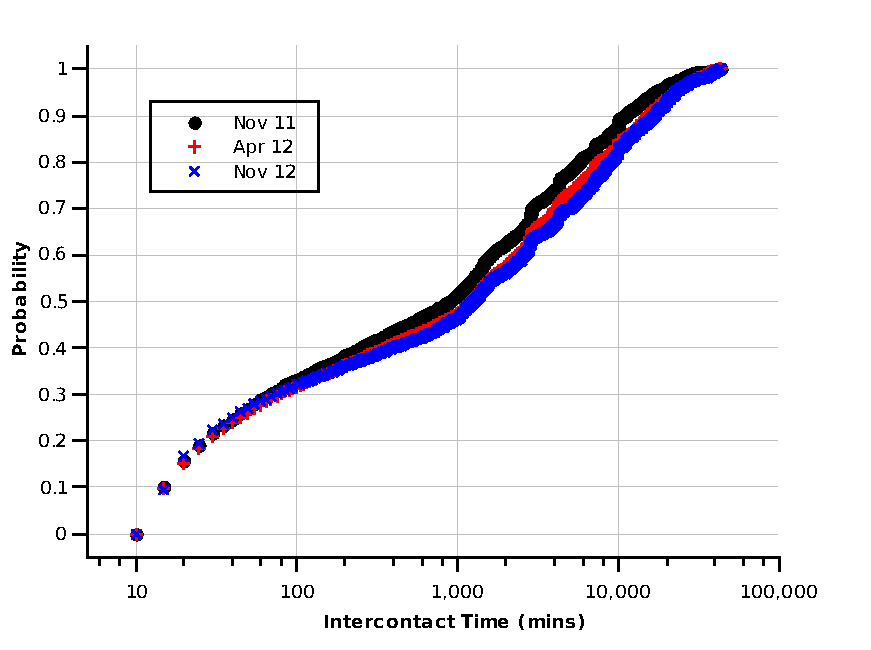
\includegraphics[width=3.5in]{graphs/intercontact_cdf.pdf}}
\caption{Intercontact Time ECDF} 
\label{fig:intercontact_cdf}
\end{figure}

\subsubsection{Measuring Effective Utility}
The final aspect for prevalence is the notion of effective utility, namely that the opportunity must occur when it is actually needed.  From a general perspective, that need can happen when the following two conditions are satisfied: a) the node $MN_i$ has some traffic to receive or send but no direct / poor connection is available  b) there is some other node $MN_j$ in proximity which can work together with the node. We analyze how often the devices really need relaying in the following three types of context. 

In order to find the appropriate range values for reasonable WiFi performance, we conducted experiments to evaluate the cutoff points of WiFi RSSI on the particular Android handset employed (Nexus S).  Channels were selected to be orthogonal to campus WiFi deployments (via a specially marked research channel space for our building) with distance, orientation, and other factors varied to get a wide variety of channel characteristics.  Downloads were conducted over 100 times for each particular configuration and the results explored for throughput.  Based on the experiment results of AP RSSI values and the corresponding throughputs, we note that -80 dBm can be the threshold to indicate good link quality with throughputs dramatically ramping up shortly after -80 dBm. At the same time, according to the RSSI distribution in Figure~\ref{fig:rssi}, there are more than 40\% of records showing that APs in campus having RSSI values larger than -80 dBm.  Therefore, we use -80 dBm as the good RSSI threshold to indicate good WiFi connection.  

The first context is when the device has traffic but does not have good WiFi connection. Figure~\ref{fig:traffic_80} includes two sets of results in Nov 2012: one is the percentage of having traffic and the other is the percentage of having traffic but the device does not have good WiFi connection (all the detected access points have signal strength less than -80dBm). Based on the results, there are more than 80\% of time slots have traffic while 30\% among them do not have good WiFi connection to do the transmission. Without WiFi, the traffic goes through the mobile link which further imposes pressure on mobile networks. However, relaying can work as an alternative to do the traffic offloading. 

\begin{figure}[tbp]
\centering 
{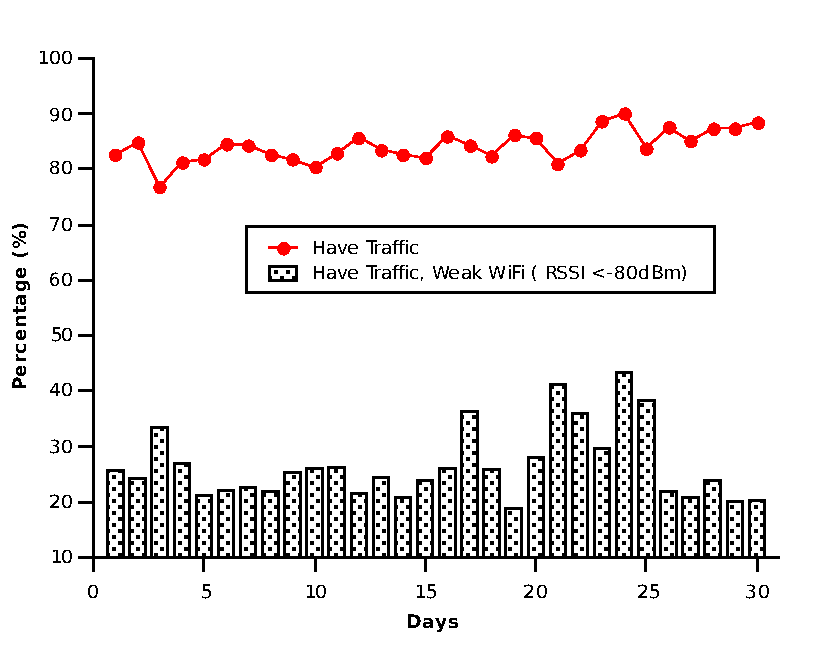
\includegraphics[width=3.5in]{graphs/traffic_80.pdf}}
\caption{Weak WiFi Signal \& Traffic} 
\label{fig:traffic_80}
\end{figure}

The second context is from the aspect of WiFi RSSI. With the prevalence of WiFi, it is interesting to investigate how often devices are not be fully covered by WiFi, i.e., detect no WiFi access points with RSSI larger than -80dBm. In such case, relay is an option. In Figure~\ref{fig:80_relay}, nearly 40\% of the time the devices do not in good WiFi environment on average. Among these time slots, there are around 20\% of them do have relaying node(s) around. 

\begin{figure}[tbp]
\centering 
{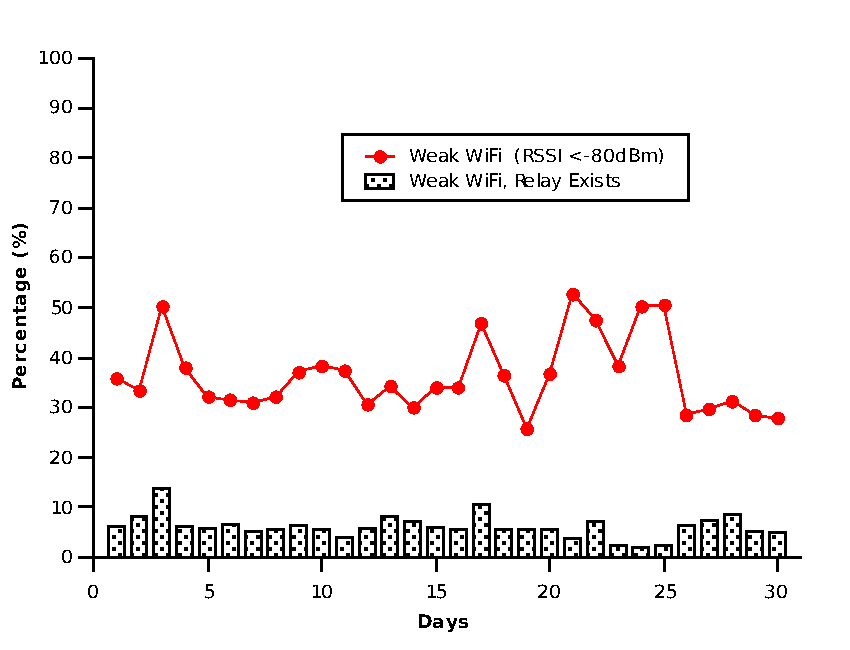
\includegraphics[width=3.5in]{graphs/80_relay.pdf}}
\caption{Relaying \& Weak WiFi Signal} 
\label{fig:80_relay}
\end{figure}

In the third context, we consider the further benefits which relaying may produce. Besides WiFi and mobile network, relaying provides the third option to transmit traffic. When there is traffic need, the device may use relaying even it has established WiFi connection. Such cases happen when the relaying nodes have the content the device requests or the relaying communication has better link quality. Based on the results shown in Figure~\ref{fig:relay_traffic}, the percentage is pretty high when relaying exists and there is traffic at the same time. Therefore, relaying can provide great opportunities for devices to send and receive traffic, not only in a passive way, but also in a proactive way. 

\begin{figure}[tbp]
\centering 
{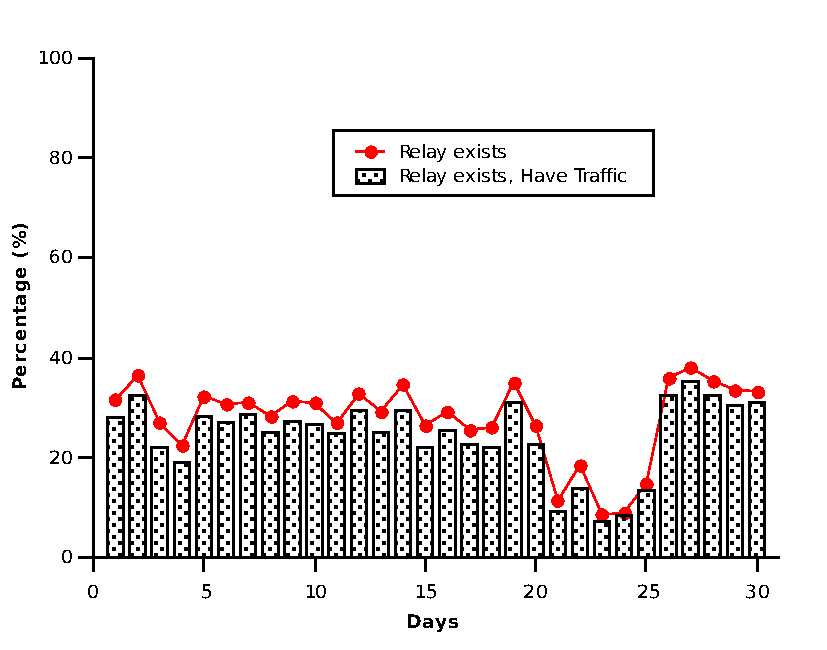
\includegraphics[width=3.5in]{graphs/relay_traffic.pdf}}
\caption{Traffic \& Relaying} 
\label{fig:relay_traffic}
\end{figure}

\subsubsection{Evaluating Prevalence} 

To summarize, we conclude our explorations on prevalence with a brief discussion of metrics and conditions used to evaluate prevalence, i.e. the potential for opportunistic communications.  

\begin{itemize}
	\item Time in Proximity: It is the most important metric for prevalence and the premise for opportunistic communication. Without enough time in proximity, any relaying protocols cannot be deployed in practice. Through the analysis of data collected from nearly 200 smartphones in the campus environment, we demonstrate such prevalence is significant. 
	\item Intercontact time: As mentioned in the last section, intercontact time is the time duration between two continuous meets for a given pair of devices. It is another characterization to indicate the frequency with which data can be transferred between networked devices.  While relevant for approaches such as DTNs, intercontact time has less relevance for single hop relaying or collaborative opportunistic communications.  
	\item Effective Utility: The prevalence of opportunities offer little utility to the handset if said prevalence occurs when the device has or no data to send, i.e. those opportunities need to occur where and when you need them.  Effective utility measures the cases where traffic demand exists and appropriate conditions exist to deliver improved wireless performance.       
\end{itemize} 

\subsection{Stability}

Prevalence becomes of little use if the set of devices available for opportunistic communications are constantly in flux.  While traditional opportunistic networking approaches assume a degree of shared trust, there exists a non-zero cost for the establishment of secure point-to-point channels or at a minimum, the assurance that the device being considered for point-to-point communications is indeed legitimate.  To that end, we evaluate the data through the lens of \emph{stabilty}, namely to what extent are the devices available detected for communication likely to be available for a reasonable duration of time.  Hence, the primary measure of stability lies in the distribution of contact durations with considerations for sufficient signal strength and symmetric connectivity detection.  Put simply, candidates for opportunistic communications must exist for a reasonable duration of time on the order of minutes, not simply seconds to amortize the cost of point-to-point channel negotiation over the lifetime of the opportunity.       

In a complementary sense, trust between various devices can be realized not only through duration but also through the repeated appearances in the local proximity.  Although an individual node may have long inter-contact times individually, the fact that a node appears consistently at multiple times per day or multiple times per week for a reasonably stable period of time implies a likely social construct or external relationship between the devices.  Hence, a secondary metric for stability is the degree to which the most frequent nodes churn, i.e. are the extent to which nodes appear for opportunities uniformly distributed and infrequent or are there nodes that appear dramatically more often than other nodes, potentially allowing for extended trust to be constructed by virtue of repeat appearances (or at a minimum, the trust exchange accelerated due to prior exchanges).  

Hence, Figure~\ref{fig:duration} explores the most basic aspect of stability, namely the average duration of devices as present with regards to the locally detected nodes. Further filtering is applied where a node must have been seen at least once per day by that node for consideration for opportunistic communication. Critically, the average stability of a connection falls at roughly 6 minutes, a considerable time period for conducting the security negotiations at the front of the communication.  

\begin{figure}[tbp]
\centering 
{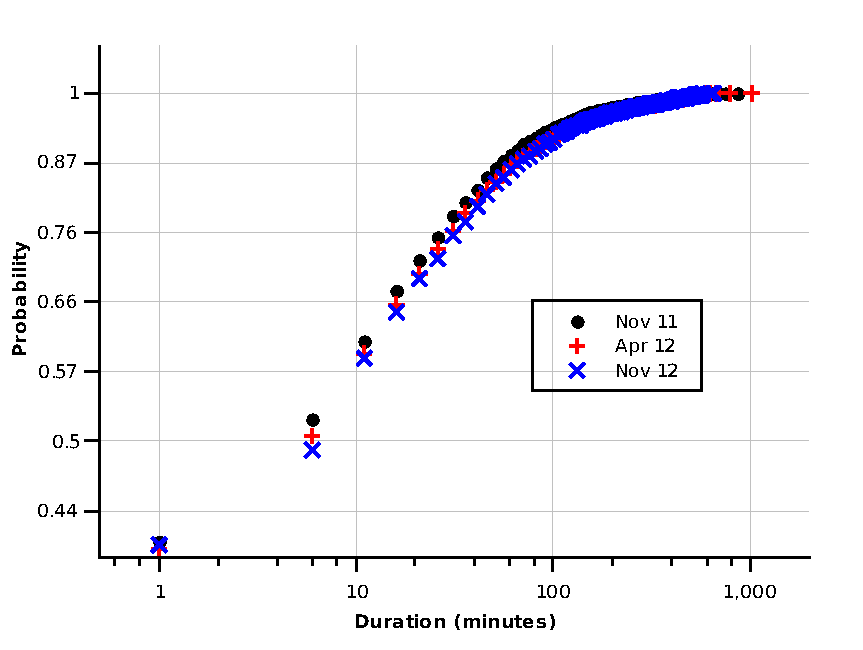
\includegraphics[width=3.5in]{graphs/duration_cdf_2.pdf}}
\caption{Proximity Duration ECDF} 
\label{fig:duration}
\end{figure}

Moreover, node strength is another metric used to evaluate the stability of proximity nodes and it is defined as follows: In one time slot, if the device detects a proximity device then the total appearance times of this peer is increased by one. Node strength is the total number of appearances of a proximity device in the period. Based on the data across 15 months, we get the node strength of proximity nodes for devices and analyze the relationship between number of relays and node strength in Figure~\ref{fig:node_strength_all}. Using the threshold of 500 for node strength, we remove those infrequent proximity nodes and calculate the average node strength for each device. It is interesting that most of the nodes have less than 10 frequent proximity nodes (loosely correlating with their social circles) and the corresponding average node strength is relatively higher than those with more than 10 frequent relays. 

\begin{figure}[tbp]
\centering 
{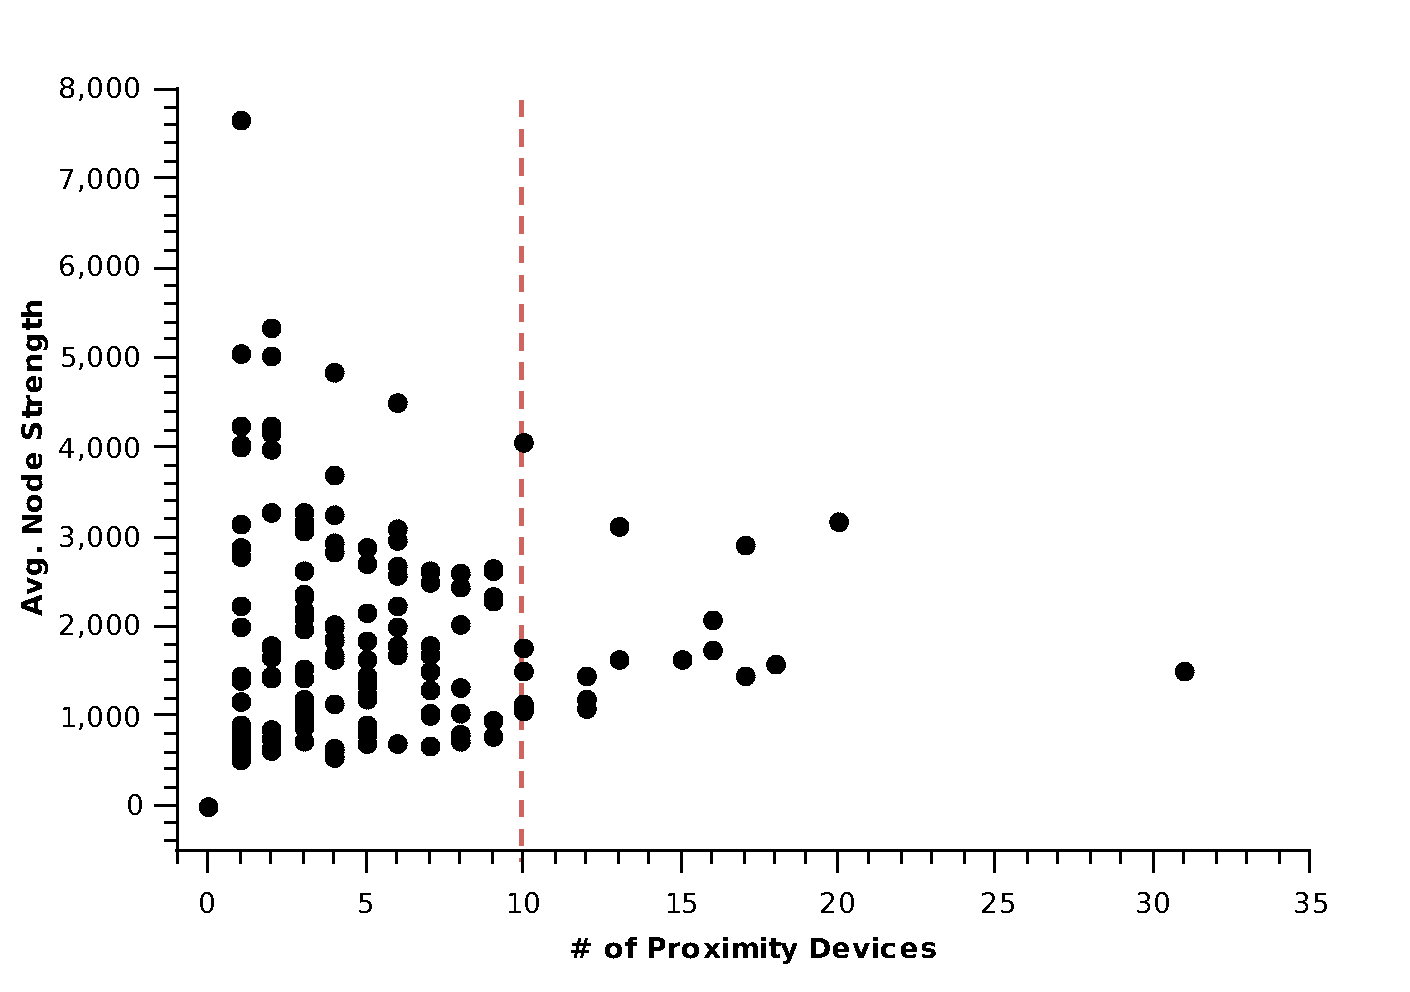
\includegraphics[width=3.5in]{graphs/node_strength_all_tag.pdf}}
\caption{Number of Proximity Nodes vs. Node Strength } 
\label{fig:node_strength_all}
\end{figure}

While node strength captures the raw magnitude of total time spent together and indirectly infers longitudinal behavior, Figure~\ref{fig:total_continuous_cdf} takes the concept further by examining the `streakiness' over multiple days by which a potential peer is likely to appear across the entire duration of the study. The total appearances represents the distribution of how frequently a node is likely to appear whereby if the prospective peer is seen at least once in the day, it counts as being successfully seen for the purposes of consistency. Note that for the purposes of the graph, all nodes are considered rather than only the nodes with a reasonable degree of consistency to capture the full longitudinal nature of the study. No filtering is done either for sufficiency of signal strength. Interestingly, several nodes eclipse nearly two-thirds of the time in the study in terms of consistency of meeting.  It is those nodes that appear consistently that represent the stable foundation from which the prevalence can be effectively leveraged.
The other plot in the graph captures the distribution of continuous days, namely if a node appears more than one day in a row, how long is the streak likely to continue with subsequent appearances over the next few days? The average number of continuous days is 1 day which means over 50\% of the proximities did not happen continuously by day.    

\begin{figure}[tbp]
\centering 
{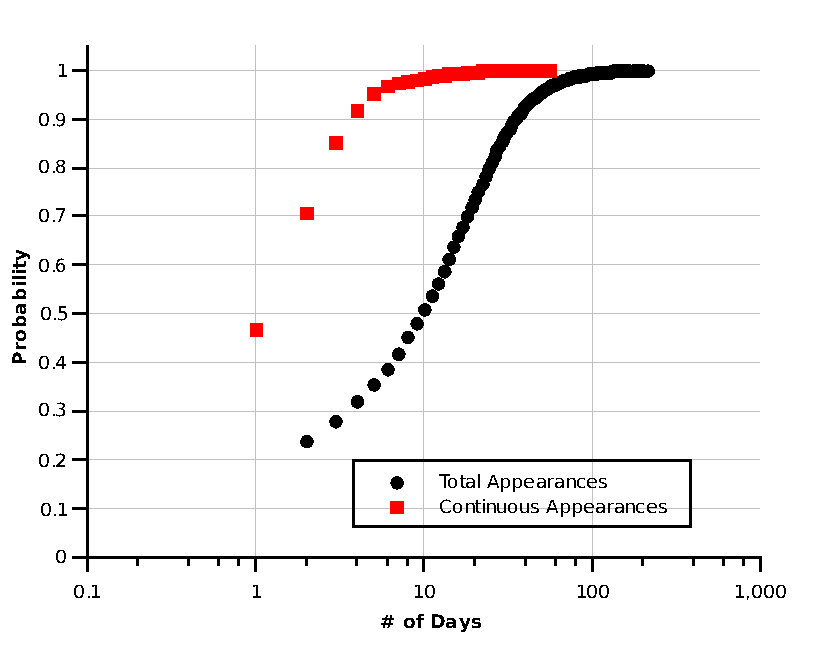
\includegraphics[width=3.5in]{graphs/total_continuous_cdf.pdf}}
\caption{Total Appearances and Continuous Appearances in Day Counts ECDF}
\label{fig:total_continuous_cdf}
\end{figure}

From the perspective of number of proximity devices, we calculate the cumulative number and compare it with the indeed active number to analyze the stability of prospective relays. The cumulative number is defined as the total number of distinguished relays in history while the weekly active number is the total number of relays which appear in the current week and were active in the past one month. Figure~\ref{fig:cumulative_active} illustrates the weekly cumulative number and active number across 15 months. The cumulative number increases to a limit (nearly the total number of devices within the project) and such value is quite stable in the following months. Meanwhile, the active number decreases across the study and big decreases happen when semesters change.  

\begin{figure}[tbp]
\centering 
{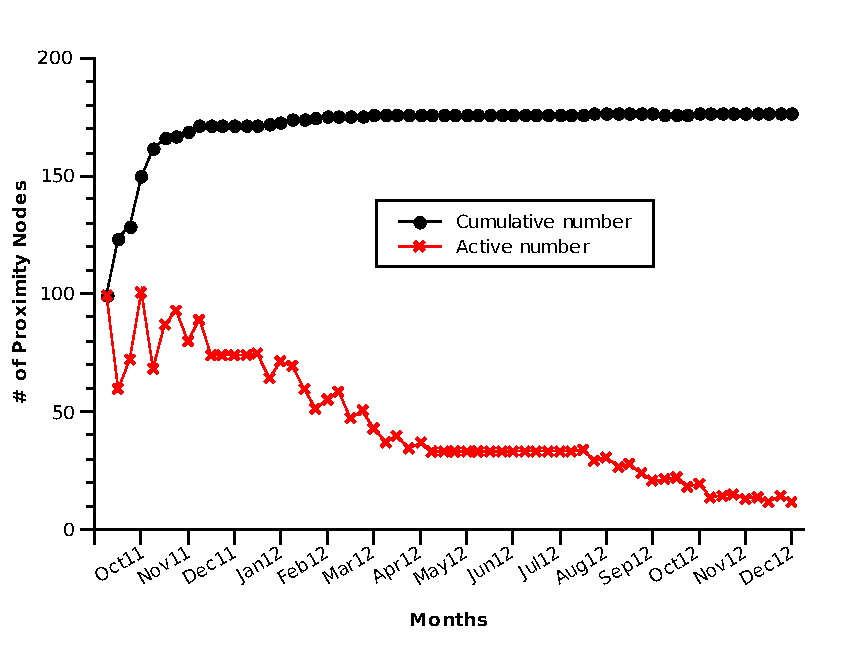
\includegraphics[width=3.5in]{graphs/cumulative_active.pdf}}
\caption{Weekly Cumulative Number and Active Number} 
\label{fig:cumulative_active}
\end{figure} 

Therefore, there are four important points for the evaluation of stability:

\begin{itemize}

\item Duration: The duration of relaying connection is essential for successful traffic transmission between the device and its relaying nodes. If two devices come across each other and separate soon, such proximity is not suitable for the establishment of usable connection. We roughly define a mean average of duration as needing to be an order of magnitude or better versus trust establishment for the mobile-to-mobile link.

\item Node Strength: The usage of node strength can capture the degree to which a trusted subset of mobile peers emerge that have the potential for expedited trust for opportunistic efforts (i.e. negotiate heavy once, light weight for the next $N$ times).

\item Total Appearances: While a purely opportunistic network where a de facto sense of trust exists can tolerate frequent dynamics in terms of random nodes serving as relay or collaboration partners, consistency of the peering partner for a node can both elicit trust by virtue of familiarity (repetition) which also has roots in normative social structures. 

\item Continuous Appearances: Although trust can be more easily inferred by virtue of repetition, consistent trust over continuous days likely implies a stronger degree of trust (not a guarantee, simply more likely). The continuous consistency ($\geq 1 /$day, $\geq 1 / $ week) can serve as a complementary metric to the earlier aforementioned inter-contact time espoused in traditional opportunistic network evaluations.
\end{itemize}

\subsection{Reciprocity}

Finally, a key metric for evaluating the potential opportunistic communication is the degree to which reciprocity exists, ideally converging to an equal ratio of service versus need.  Although altruism amongst nodes typically leads to a healthier network performance as a whole, the potential for increased energy consumption is of little consolation if the device is always helping but never benefitting.  To that end, we posit that reciprocity amongst nodes must be taken into account when considering the overall utility of an opportunistic solution.  Whereas much of the prior work is limited to evaluating only some aspects of prevalence and stability, interactions among pairs (dyads) in the study afford us the ability to evaluate the extent to which reciprocity exists both in short and long-term time scales with actual traffic patterns and actual energy constraints.  

To that end, Figure~\ref{fig:reciprocal} shows the daily average percentages with respect to needing assistance (relaying to another node) versus offering assistance (relaying for another node).  The data is drawn strictly from intra-study interactions across the month of November 2012.  A mobile node is defined as needing assistance if it has traffic but detects no WiFi access points with a sufficient signal strength ($> -80 dBm$).  A mobile node is defined as serving (offering assistance) if it has a good WiFi connection and has been detected by other nodes within the study.  Hence, a value of 25\% with respect to being detected as a relay denotes that another node ($MN_j$) in the study detected the node ($MN_i$), $MN_j$ had a good signal strength to the node $MN_i$, and $MN_i$ had a good signal strength for WiFi for 25\% of the time that $MN_i$ was on for that day.  Critically, a node needing relaying but detecting no nodes is similar to a node being willing to serve but yet no nodes needing its service. A further sub-division is done to breakdown the nodes filtered if battery level were taken into consideration, i.e. what percentage could no longer offer assistance if the battery level fell below 30\% which barely has an impact, typically only a reduction of 1-3\% for the number of times a node could offer assistance but would not due to energy constraints.   

\begin{figure}[tbp]
\centering 
{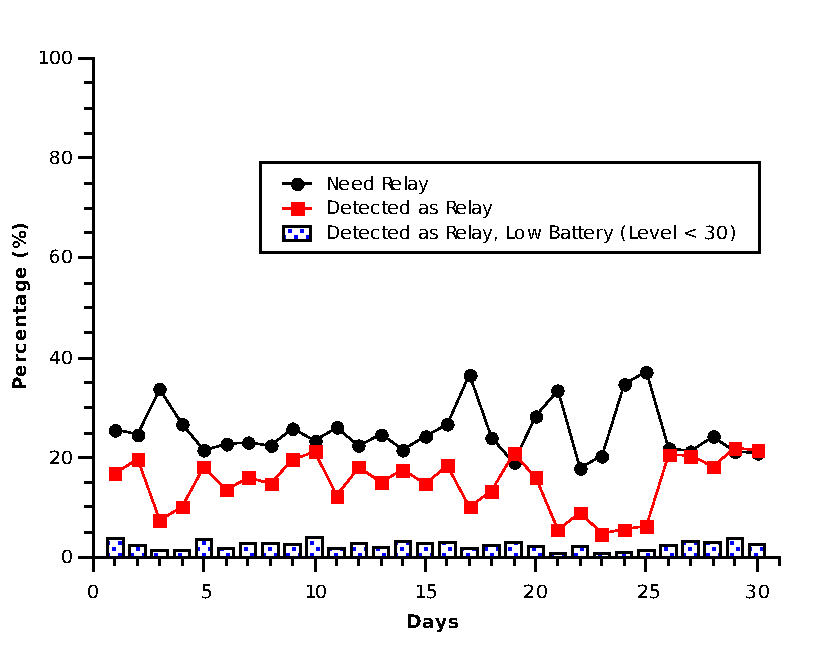
\includegraphics[width=3.5in]{graphs/reciprocal.pdf}}
\caption{Distribution of Potential Interactions - Need vs. Serve (November 2012)} 
\label{fig:reciprocal}
\end{figure} 

For a reasonable portion of the time, most nodes on average have an increased need for assistance versus the ability to serve.  The primary exceptions emerge on weekends which also happen to correspond with football games, campus events, and travel.  
Figure~\ref{fig:1117} captures this relationship on both short-term (single day) and longer-term (one week/one month) timescales drawing from a single week from Figure \ref{fig:reciprocal}.  The figure plots the distribution of the node having the potential to serve versus needing assistance.  A ratio of one implies that the node had an equal number of time slots where the node could serve as a relay (detected, good WiFi) versus the node needing a relay.   Whereas the traffic from the weekend shows much stronger need (due in part to the lack of WiFi at the football stadium), the nodes on the long-term scale have ratios much closer to 1 representing a reasonable reciprocity.  Moreover, the typical weekday (as opposed to the game day scenario with limited WiFi) gravitates more closely to a balanced distribution as well.  Similarly as diurnal analysis in Section~\ref{sec:prevalence}, the diurnal distribution of such ratio is shown in Figure~\ref{fig:diurnal_ratio}. Notably, the ratio is most balanced in daytime while the needing is more than offering due to the lack of WiFi during the night and sleep time. 

\begin{figure}[tbp]
\centering 
{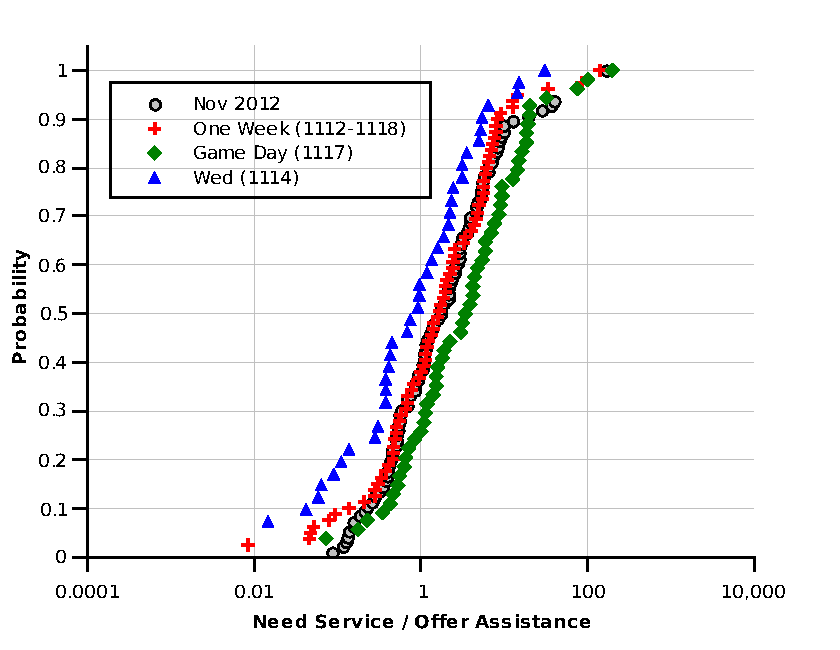
\includegraphics[width=3.5in]{graphs/1117_2.pdf}}
\caption{Ratio of Needing vs. Serving (November 2012)} 
\label{fig:1117}
\end{figure} 

\begin{figure}[tbp]
\centering 
{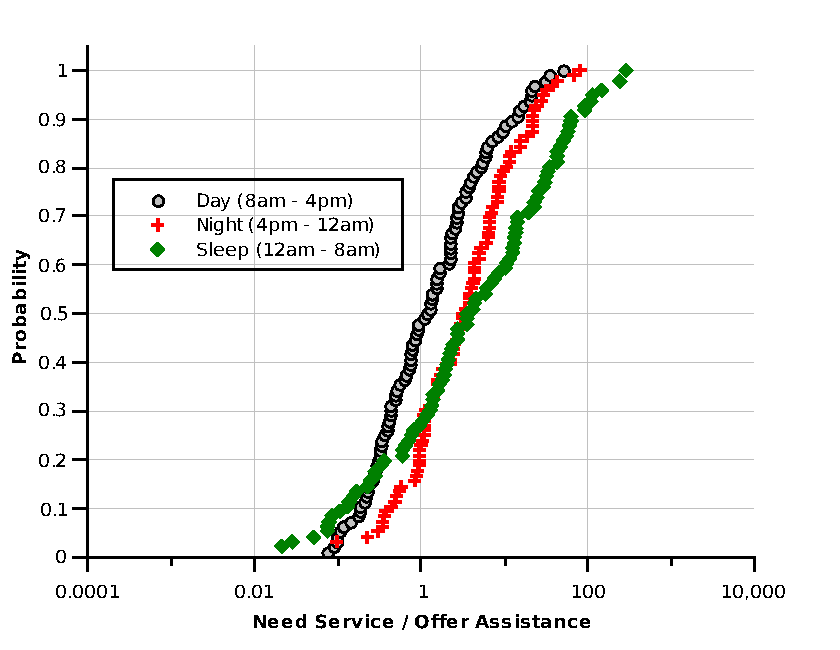
\includegraphics[width=3.5in]{graphs/diurnal_ratio.pdf}}
\caption{Diurnal Distribution of Ratio (November 2012)} 
\label{fig:diurnal_ratio}
\end{figure} 

To close, we list the essential criteria related to reciprocity and their formal definitions as follows:

\begin{itemize}

\item Needs Service: A critical first step to establishing the likely reciprocity is to characterize the share of time that a node is in the need service state, namely does the node either have poor / none WiFi or alternatively poor / no cellular coverage. The need service case is where the node will perceive value to the underlying opportunistic communications.

\item Offers Assistance: In contrast to needing service, the ability to offer service represents the altruistic aspects of needing service, namely when can the node assist other nodes? The share of when a node can offer relaying / collaboration must be considered along with energy filters excluding devices with low energy levels.

\item Service vs. Assistance: The final and most critical component is the actual ratio of reciprocity itself, ex. how often is the device likely to serve versus the device need service? While atypical situations can exacerbate sharing (everyone needs help), the normative situation should be one where reciprocity is preserved both on short-term timescales (daily) and long-term timescales (weekly, monthly).

\end{itemize}

\section{Summary}

Critically, we investigate the availability of opportunity for relaying and demonstrate that not only is such opportunity more prevalent than expected, the opportunities are stable enough to be worthwhile to establish even with auxiliary security constraints and the opportunities are reciprocal across both short-term and long-term time scales even when considering energy levels of the involved devices. Specifically, the key contributions are as follows:

\begin{itemize}
	\item \emph{Investigate the availability of opportunity for relay:} Proximity among mobile devices is the key to determine whether relaying can happen or not. Based on  Bluetooth and WiFi detections, we are able to use appropriate signal strength to reflect the relative distance of devices. Moreover, power is essential for mobile devices therefore residual battery is another important fact to be considered for availability.
	 
	\item \emph{Demonstrate the opportunity (prevalence) for relaying is indeed significant:} Through the analysis of a 15 month dataset of detailed smartphone data gleaned from nearly 200 smart phone users, we demonstrate that a typical user can find devices amenable to relaying averaging nearly 60\% of the time. To the best of our knowledge, we believe our study is the first to conduct a longitudinal study of relaying prevalence with demonstrating ample opportunities with respect to both raw relaying prevalence and useful relaying prevalence .  

	\item \emph{Demonstrate that said opportunities for relaying are not only prevalent but stable:} We show with our study data that relaying opportunities existing on average for durations of 6+ minutes. Moreover, we show that the opportunities for relaying tend to be highly focused on a select subset of devices enabling enhanced levels of trust versus random, intermittent opportunities as espoused in the literature.  

	\item \emph{Demonstrate that said opportunities would largely be reciprocal:} In addition to opportunities being prevalent and stable (useful), we show that interactions for relaying would be overwhelmingly reciprocal in both short-term and long-term time windows, even when accounting for the energy levels of both parties involved in the relaying.  We demonstrate this through the inclusion of actual traffic demands on fine temporal granularities, a unique feature of our dataset.  

	\item \emph{Propose a framework to evaluate the relaying potential for network traces:} While we believe our work is one of the first of its kind to fuse fine-grained proximity and traffic data over such a long period, we hope that others will embark on similar efforts to broaden the effective data pool available to the community.  To that end, we view all of our data through the lens of what we dub the APSR (Availability, Prevalence, Stability, Reciprocity) framework, a framework for systematically evaluating the potential and quality of the proximity of mobile network trace data.  
\end{itemize}

